\documentclass{article}
\usepackage{amsmath,amsfonts,amsthm,amssymb,amsopn,bm}
\usepackage[margin=.9in]{geometry}
\usepackage{graphicx}
\usepackage{url}
\usepackage[usenames,dvipsnames]{color}
\usepackage{fancyhdr}
\usepackage{multirow}
\usepackage{listings}
\usepackage{hyperref}

\definecolor{keywords}{RGB}{255,0,90}
\definecolor{comments}{RGB}{0,0,113}
\definecolor{red}{RGB}{160,0,0}
\definecolor{green}{RGB}{0,150,0}
 
\lstset{language=Python, 
        basicstyle=\ttfamily\tiny, 
        keywordstyle=\color{keywords},
        commentstyle=\color{comments},
        stringstyle=\color{red},
        showstringspaces=false}

\newcommand{\field}[1]{\mathbb{#1}}
\newcommand{\1}{\mathbf{1}}
\newcommand{\E}{\mathbb{E}} 
\newcommand{\Z}{\mathbb{Z}} 
\renewcommand{\P}{\mathbb{P}}
\newcommand{\R}{\field{R}} % real domain
% \newcommand{\C}{\field{C}} % complex domain
\newcommand{\F}{\field{F}} % functional domain
\newcommand{\T}{^{\textrm T}} % transpose
\def\diag{\text{diag}}

%% operator in linear algebra, functional analysis
\newcommand{\inner}[2]{#1\cdot #2}
\newcommand{\norm}[1]{\left\|#1\right\|}
\newcommand{\twonorm}[1]{\|#1\|_2^2}
% operator in functios, maps such as M: domain1 --> domain 2
\newcommand{\Map}[1]{\mathcal{#1}}
\renewcommand{\theenumi}{\alph{enumi}} 

\newcommand{\Perp}{\perp \! \! \! \perp}

\newcommand\independent{\protect\mathpalette{\protect\independenT}{\perp}}
\def\independenT#1#2{\mathrel{\rlap{$#1#2$}\mkern2mu{#1#2}}}
\newcommand{\vct}[1]{\boldsymbol{#1}} % vector
\newcommand{\mat}[1]{\boldsymbol{#1}} % matrix
\newcommand{\cst}[1]{\mathsf{#1}} % constant
\newcommand{\ProbOpr}[1]{\mathbb{#1}}
\newcommand{\points}[1]{\small\textcolor{magenta}{\emph{[#1 points]}} \normalsize}
\date{{}}

\setlength\parindent{0px}

\begin{document}
\title{Homework \#5}
\author{\normalsize{Winter 2020, STATS 509}\\
\normalsize{Dino Bektesevic}}
\maketitle


\subsection*{Problem 1}
A researcher is studying a certain population of animals. The researcher is interested in the proportion $\theta$ of females. Her prior is Beta$(\alpha, \beta)$, where $\alpha, \beta > 0$ are positive integers, 
$$ p(\theta) = \left\{ \begin{array}{cc}
    \frac{(\alpha + \beta - 1)!}{(\alpha -1)! (\beta-1)!} \theta^{\alpha-1}(1-\theta)^{\beta-1} & 0< \theta < 1,\\[6pt]
    0 & \hbox{otherwise}.
\end{array}
\right.
$$
The researcher conducts two studies. In the first study she obtains a random sample of size $n$ in total, that contains $f$ females and $m$ males. 
\begin{enumerate}
    \item[(a)] Find the density for the researcher's posterior distribution $p(\theta \,|\, f,m)$ for $\theta$ after conducting the first study.\par
    {\it Hint: you may cite results from lecture notes here.}
    From class we have the posterior given by
    $$p(\theta | f,m) \approx Beta(\alpha+f, \beta+m)$$
\end{enumerate}
\noindent In the second study, the researcher randomly samples animals until she observes the first male, at which point she stops. Let $t$ be the total number of animals (both male and female) sampled in the second study.
\begin{enumerate}
    \item[(b)] Write down the likelihood $p(t | \theta)$.
    $$L(\theta | t) = (1-\theta)\theta^{t-1}$$

    \item[(c)] Using the posterior  resulting from the first study (found in (a)) as the researcher's prior  before seeing the data from the second study, write down an expression that is proportional to the researcher's posterior density $p(\theta | t, f,m)$ after observing the data from {\bf both} studies.
    \begin{align*}
        p(\theta | t, f, m) &= p(\theta) p(t|\theta) \\
        &= \frac{(\alpha+f+\beta + m -1)!}{(\alpha + f -1)!(\beta + m -1)!}\theta^{\alpha + f - 2}(1-\theta)^{\beta + m} \\
        &\approx \theta^{\alpha + f - 2 }(1-\theta)^{\beta + m}
    \end{align*}
    
    \item[(d)] Using your answer to (c), or otherwise, find the researcher's posterior density,  $p(\theta \,|\, t, m,f)$ after both studies.
    {\bf Hint:} {\it  Recall that for $r$, $s$ positive integers,
    $$ \int_0^1 u^{r-1}(1-u)^{s-1}du  = {{(r-1)!(s-1)!}\over {(r+s-1)!}}.  $$}
    
    \begin{align*}
        1 &= \int f(p|x) dx \\
        &= c\int_0^1 \theta^{\alpha+f+t-2}(1-\theta)^{\beta + m}d\theta \\
        &= c \frac{(\alpha + f + t -2)! (\beta+m)!}{(\alpha + f + t + \beta + m -1)!} \\
        c &= \frac{(\alpha + f + t + \beta + m -1)!}{(\alpha + f + t -2)! (\beta+m)!}
    \end{align*}
    
    \item[(e)] Using the definition of expectation, or otherwise, find $E[\theta \,|\, t, m, f]$, the mean of the researcher's posterior distribution.
    
    \begin{align*}
        E[\theta | t, m, f] &= \int_0^1 \theta f(\theta| t, m, f) d\theta \\
        &= \frac{(\alpha + f + t + \beta + m -1)!}{(\alpha + f + t -2)! (\beta+m)!} \int_0^1 \theta^{\alpha + f + t -1}(1-\theta)^{\beta+m} d\theta \\
        &= \frac{(\alpha + f + t + \beta + m -1)!}{(\alpha + f + t -2)! (\beta+m)!}  \frac{(\alpha + f + t -1)!(\beta+m)!}{(\alpha + f + t +\beta + m)} \\
        &= \frac{(\alpha + f + t + \beta + m -1)!}{(\alpha + f + t -2)!}  \frac{(\alpha + f + t -1)!}{(\alpha + f + t +\beta + m)} \\
        &= \frac{\alpha + f + t -1}{\alpha + f + t +\beta + m}
    \end{align*}

    \item[(f)] Suppose that another researcher had the same prior, Beta$(\alpha, \beta)$, but then learned about the results of both studies  ($t,m,f$) simultaneously. Show that the posterior which results will be the same as in (d).\par
    {\it Hint: note that because the studies are independent (given $\theta$), $p(t,f,m\,|\,\theta) = p(t\,|\,\theta)p(f,m\,|\,\theta)$.}
\end{enumerate}


\newpage
\subsection*{Problem 2} 
Suppose that we have a Beta$(1,1)$ prior for $p$, the mean of a Bernoulli random variable.
\begin{enumerate}
        \item[(a)] Find the density for $\psi = p(1-p)$, the variance of a Bernoulli random variable. (Hint: use the CDF method.) Plot this density.
    
    \begin{align*}
        P(\psi \leq t) &= P(p(1-p) \leq t) \\
        &= P(p-p^2 \leq t) \\
        &= P(-p^2 + p -t \leq 0) \\
        &= P\left( p \leq \frac{1}{2} - \sqrt{\frac{1}{4} - t}\right) + P\left( p \geq \frac{1}{2} + \sqrt{\frac{1}{4} - t}\right)
    \end{align*}
    The above expression are essentially CDFs and since $p\approx Beta(1,1)$, which is uniform over [0,1], we can just say that
    $$P(\psi \leq t) = 1- 2\sqrt{\frac{1}{4} - t}$$
    
    The pdf then is:
    
    \begin{align*}
        f(\psi = t) &= \frac{\partial}{\partial t} F(t) \\
        &= \left(\frac{1}{4} - t\right)^{-\frac{1}{2}} \\
        &= \frac{1}{\sqrt{\frac{1}{4} - t}}
    \end{align*}
    for $t\in [0, \frac{1}{4}$
    
    \begin{center}
        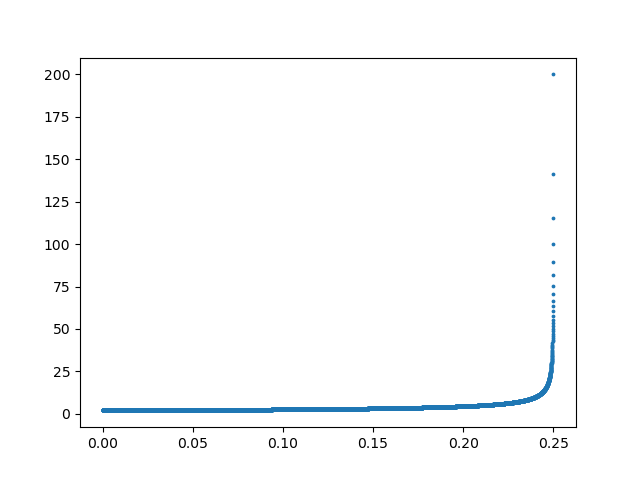
\includegraphics[width=0.5\textwidth]{STATS509/HW6/HW6Figures/problem2a.png}
    \end{center}
    
    \item[(b)] The Beta$(1,1)$ density for $p$ has sometimes been claimed to be a `non-informative' prior, i.e.~representing a state of belief corresponding to knowing `nothing'. Using the plot from (a) comment briefly on this claim. 
    
    Non-informative priors don't exactly correspond to knowing "nothing", but instead to the belief that $p$ is equally probable to be any value from 0 to 1. Given this assumption we can see from the plot that variance of $V(\theta)$ is not uniform too, but that, given that assumption, more likely to be larger than, lets say, 0.15. 
\end{enumerate}



\newpage
\subsection*{Problem 3} 
A researcher plans to record the number of mini-earthquake events $X$ occurring in a given time period near a volcano. She believes this is modelled well by a Poisson distribution with parameter $\lambda$:
    $$p(x \mid \lambda) = {{\lambda^x e^{-\lambda}}\over {x!}}\quad\quad \lambda > 0.$$
Before seeing any data, her beliefs about $\lambda$ are described by an exponential($2$) distribution which has the following pdf: 
    $$p(\lambda) = \left\{ \begin{array}{cl}
        2 e^{-2\lambda}  & \hbox{ for } \lambda > 0\\
        0 &\hbox{ otherwise,}
    \end{array}
    \right.
    $$
\begin{enumerate}
    \item[(a)] Before observing the data, with what probability does the researcher believe that $\lambda < 1$? 
    
    This is just purposefully confusingly written because in text they give $lambda = 2$ but overload the $\lambda$ with the Poisson distribution parameter one. The answer is just the CDF of the exponential prior where, not the $\lambda$ in the expression, is 2 and the $\lambda$ in the expression is 1. So:
    $$F(\lambda=1) = 1 - e^{-2\lambda} = 1 - e^-2 = 0.865$$

    \item[(b)] If the researcher observes $x_0$ earthquakes, write down an expression that is {\it proportional to} the pdf $p(\lambda \mid x_0)$ describing her beliefs about $\lambda$ after making this observation.
    
    \begin{align*}
        p(\lambda |x_0) &= p(\lambda)p(x_0|\lambda) \\
        &= 2 e^{-2\lambda} \frac{\lambda^{x_0}e^{-\lambda}}{x_0!} \\
        &\approx \lambda^{x_0} e^{-3\lambda}
    \end{align*}

    \item[(c)] Find the constant of proportionality in (b), and hence find the pdf for the researcher's posterior distribution $p(\lambda \mid x_0)$.
    {\it Hint: Note that $\int_{0}^{\infty} t^n e^{-at}dt = n!/a^{n+1}$ for $a>0$, and $n$ a positive integer.}
        
    \begin{align*}
        1 &= C \int \lambda^{x_0} e^{-3\lambda} \\
        &= C \frac{x!}{3^{x+1}} \\
        C = \frac{3^{x+1}}{x!}
    \end{align*}
    
    \item[(d)] Suppose that no earthquakes occur, and so $x_0=0$. Use your answer in (c) to find the probability with which the researcher now believes that $\lambda < 1$. What do you notice?
    
    $$p(\lambda | x_0 = 0) = 3 e^{-3\lambda}$$
    
    Keeping in mind the confusion about $x$ vs $\lambda$ in the notation, we see this is an exponential distribution with the parameter $\lambda=3$ so evaluating a CDF for less than or equal to 1 occurrence gets us:
    $$F(\lambda=1) = 1 - e^{-3\lambda} = 1 - e^{-3} = 0.95$$
    a rather high probability of one or less events.
\end{enumerate}


\newpage
\subsection*{Problem 4}

Suppose that we have a sample of size $n$ from a Normal distribution with mean $\mu$, variance $\sigma^2$, where $\sigma^2$ is known. The observed mean for the sample is $\bar{x}$.
\begin{enumerate}
    \item[(a)] Write down the density for $f(\bar{x} \mid \mu)$.  This is the likelihood for $\bar{X}$ given $\mu$ (see note below).
    {\it (Hint: see Goldberger Section 8.3)}
    
    \item[Fact] (Useful for part (b)) Note that if
    $$h_1(\theta) = {1\over {a^2}} (u-\theta)^2 \quad\quad\quad  h_2(\theta) = {1\over{b^2}} (v-\theta)^2$$ 
    and $h(\theta) = h_1(\theta) + h_2(\theta)$, then
    $$h(\theta) = {({1\over {a^2}}+{1\over{b^2}})}\left({{{u\over {a^2}}+{v\over{b^2}}}\over {{1\over {a^2}}+{1\over{b^2}}}} - \theta \right)^2 + c$$
    where $c$ is a constant (i.e. it does not depend on $\theta$.)\par
    {\it You do not need to prove this.}

    \item[(b)] Suppose that our prior distribution for $\mu$ is N$(\mu_0,\tau_0^2)$, so 
    $$f(\mu) = {1\over{\sqrt{2\pi} \tau_0}}e^{-{1\over {2\tau_0^2}} (\mu-\mu_0)^2}$$
    where $\mu_0$ and $\tau_0^2$ are known constants. Verify the expression given for the posterior distribution of 
    $$\mu \mid \bar{x}$$
    in the last slide of Lecture 9.\\[16pt]
    {\it Hint: remember that by Bayes' rule:
    $$f(\mu \mid \bar{x}) \propto f(\bar{x} \mid \mu) f(\mu)$$
    and use the expression derived in (b). It is also sufficient to simply `spot' the form of the density. i.e. observe that $f(\bar{x} \mid \mu) f(\mu)$ is proportional to a given known density. Thus no integration is required to answer this question.}
\bigskip

 
{\small {\bf\small  Note:} to keep the notation simple above I have suppressed conditioning on the
known population variance $\sigma^2$ e.g.~the likelihood could be
written as: $p(\bar{x} \mid \mu, \sigma^2)$, the prior on $\mu$ would then also be written
as $p(\mu \mid \sigma^2)$. A strict Bayesian might prefer to condition explicitly
on the constants to make clear what was being assumed known.\par
{\it This is a philosophical/ notational issue that is not directly relevant to the
calculation you are asked to make in the question above.}\par
}
% (Also $n$ in question 2.)}
\end{enumerate}


\newpage
\subsection*{Bayesian inference for a Normal mean with unknown variance and independent priors}
\noindent Read the following notes before attempting Qu. 5:
 
\hspace{-1cm}{\scriptsize \url{https://www.stat.washington.edu/tsr/s509/lecture9f02/notes-on-normal-mean-variance.pdf}}\par
\hspace{-1cm}{\scriptsize \url{https://www.stat.washington.edu/tsr/s509/lecture9f02/Bayesian-mean-var-for-normal-with-R.pdf}}\par
\medskip

\noindent{\it\small (For people who would like to use Python, it should be feasible to implement this using the two notes above as a guide.)}


\subsection*{Problem 5} 
On three days between July 24 and September 5, 1882 the physicist Simon Newcomb measured the amount of time it took light to travel from his lab, to a mirror on the Washington Monument, and back to his lab. The data are here:

\hspace{-1cm}{\scriptsize \url{https://www.stat.washington.edu/tsr/s509/examples/newcomb/newcomb-light-data.csv}}

Use the following lines of R to read in the data and put the observed times into a vector $y$:%
{\small
\begin{verbatim}
newcomb <- read.table('newcomb-light-data.csv',header=TRUE,sep=",")
y <- newcomb$time
\end{verbatim}}%
{\small (The experiments were conducted over three days, recorded in {\tt newcomb\$day}; we will not use this here.)}

The times are in microseconds (s$\times 10^{-6}$) (millionths of a second); the distance of the path traveled is $7.44373$ km.  

Suppose that the observations $Y_1,\ldots ,Y_{n}$ are i.i.d.~samples from a population with $N(\mu,\sigma^2)$; where $\mu$ is the time it takes light to travel along the path and $\sigma^2$ describes variability due to experimental error.

There had been prior experiments by Fizeau and Foucault that attempted to measure the speed of light. Suppose that Newcomb's beliefs regarding $\mu$ were described as follows:
\begin{eqnarray*}
    \mu &\sim& N(\mu_0,1/\tau_0^2)
\end{eqnarray*}
where $\mu_0=30$ and $\tau_0^2=0.01$. Thus under his prior 
$$P( \mu \in [30 -1.96/\sqrt{0.01}, 30 +1.96/\sqrt{0.01}])  = P( \mu \in [10.4, 49.6]) = 0.95.$$ 
Further suppose that his prior on $\sigma^2$ was described as follows:
\begin{eqnarray*}
    1/\sigma^2 = \phi^2 &\sim & \hbox{Gamma}(\nu_0/2, \nu_0/(2\phi_0^2)) = \hbox{Gamma}(1/2, 1/2)
\end{eqnarray*}
so $\nu_0=1, \phi_0^2 =1$. (Equivalently this is a Chi-square distribution with $1$ d.f.) This prior puts high probability on $\phi^2$ being close to $0$, or equivalently, on $\sigma^2$ being large, indicating large error.

Since prior information about $\mu$ would come from work by others on the speed of light, while information relating to $\sigma^2$ pertains to Newcomb's set-up, which was new, it is reasonable to think that the priors on $\mu$ and $\sigma^2$ (or equivalently on $\mu$ and $\phi^2$) would be independent.(Note that $\mu$ and $\sigma^2$ are independent under the prior if and only if $\mu$ and $\phi^2 = 1/\sigma^2$ are independent under the prior. (Why?))

{\bf Note:} Except for part (b)(vi), the questions below can all be answered by making minor edits to the script which will be {\tt mean-var-for-normal.r} covered in lab on Friday.

\newpage
\begin{enumerate}
    \item[(a)] Obtain a discrete approximation to the posterior distribution $p(\mu,\phi^2 \mid y_1,\ldots ,y_n)$. Use this to obtain:
    \begin{enumerate}
        \item[(i)] a heat-map showing the discrete approximation to the joint posterior,
        
        \begin{center}
            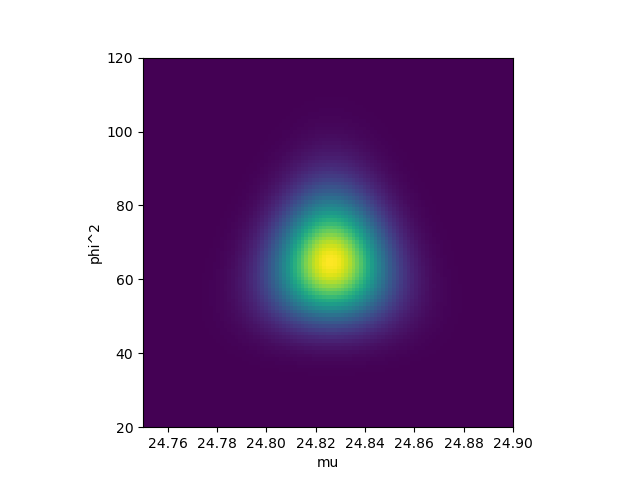
\includegraphics[width=0.5\textwidth]{STATS509/HW6/HW6Figures/problem5ai.png}
        \end{center}
        
        \item[(ii)] discrete approximations to the marginal densities, $p(\mu \mid y_1,\ldots ,y_n)$ and $p(\phi^2 \mid y_1,\ldots ,y_n)$; construct plots showing these approximations.
        
         \begin{center}
            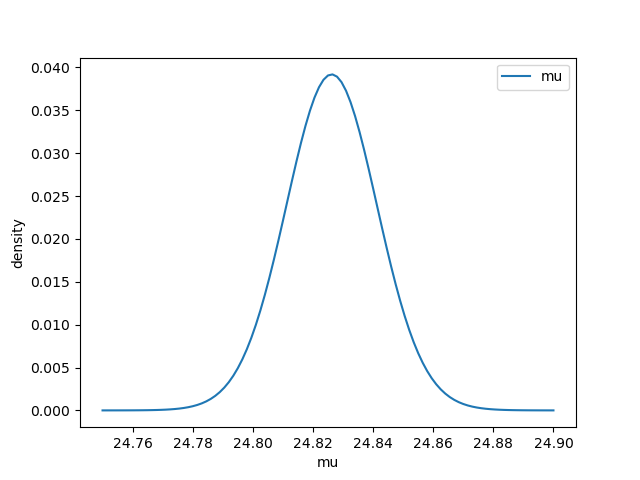
\includegraphics[width=0.4\textwidth]{STATS509/HW6/HW6Figures/problem5aii1.png}
            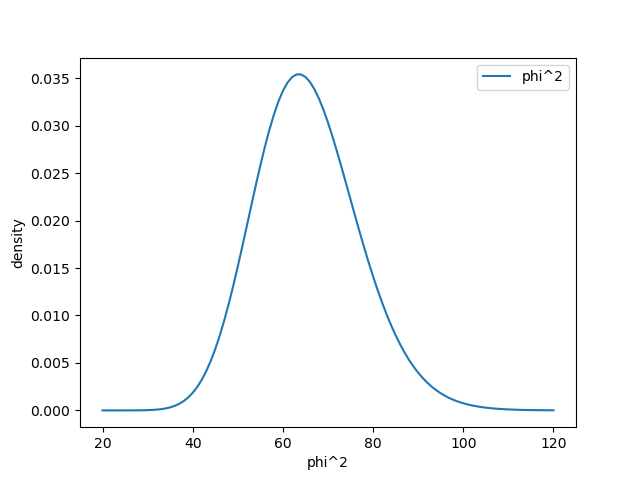
\includegraphics[width=0.4\textwidth]{STATS509/HW6/HW6Figures/problem5aii2.png}
        \end{center}
        
    \end{enumerate}
    {\it Hints: (1) check that the prior parameters {\tt mu0, tau20, nu0, phi20} corresponding to $\mu_0$, $\tau^2_0$, $\nu_0$ and $\phi^2_0$ are set correctly. (2) To find the limits for your grid of values {\tt mu.grid} and {\tt phi2.grid}, it may be useful to do part (b) below first. (3) The range for {\tt mu.grid} needs to be made quite small since the data is highly informative. (4) For the same reason the range for {\tt phi2.grid} needs to be made large (up to $100$), but should not include $0$ or negative numbers as then the density is not defined.}

    \newpage
    \item[(b)] Use the Gibbs sampler to obtain $10,000$ (dependent) draws from the posterior distribution $p(\mu,\phi^2 \mid y_1,\ldots ,y_n)$. 
    \begin{enumerate}
        \item[(i)] Construct a scatterplot showing these $10,000$ draws.
    
        \begin{center} 
            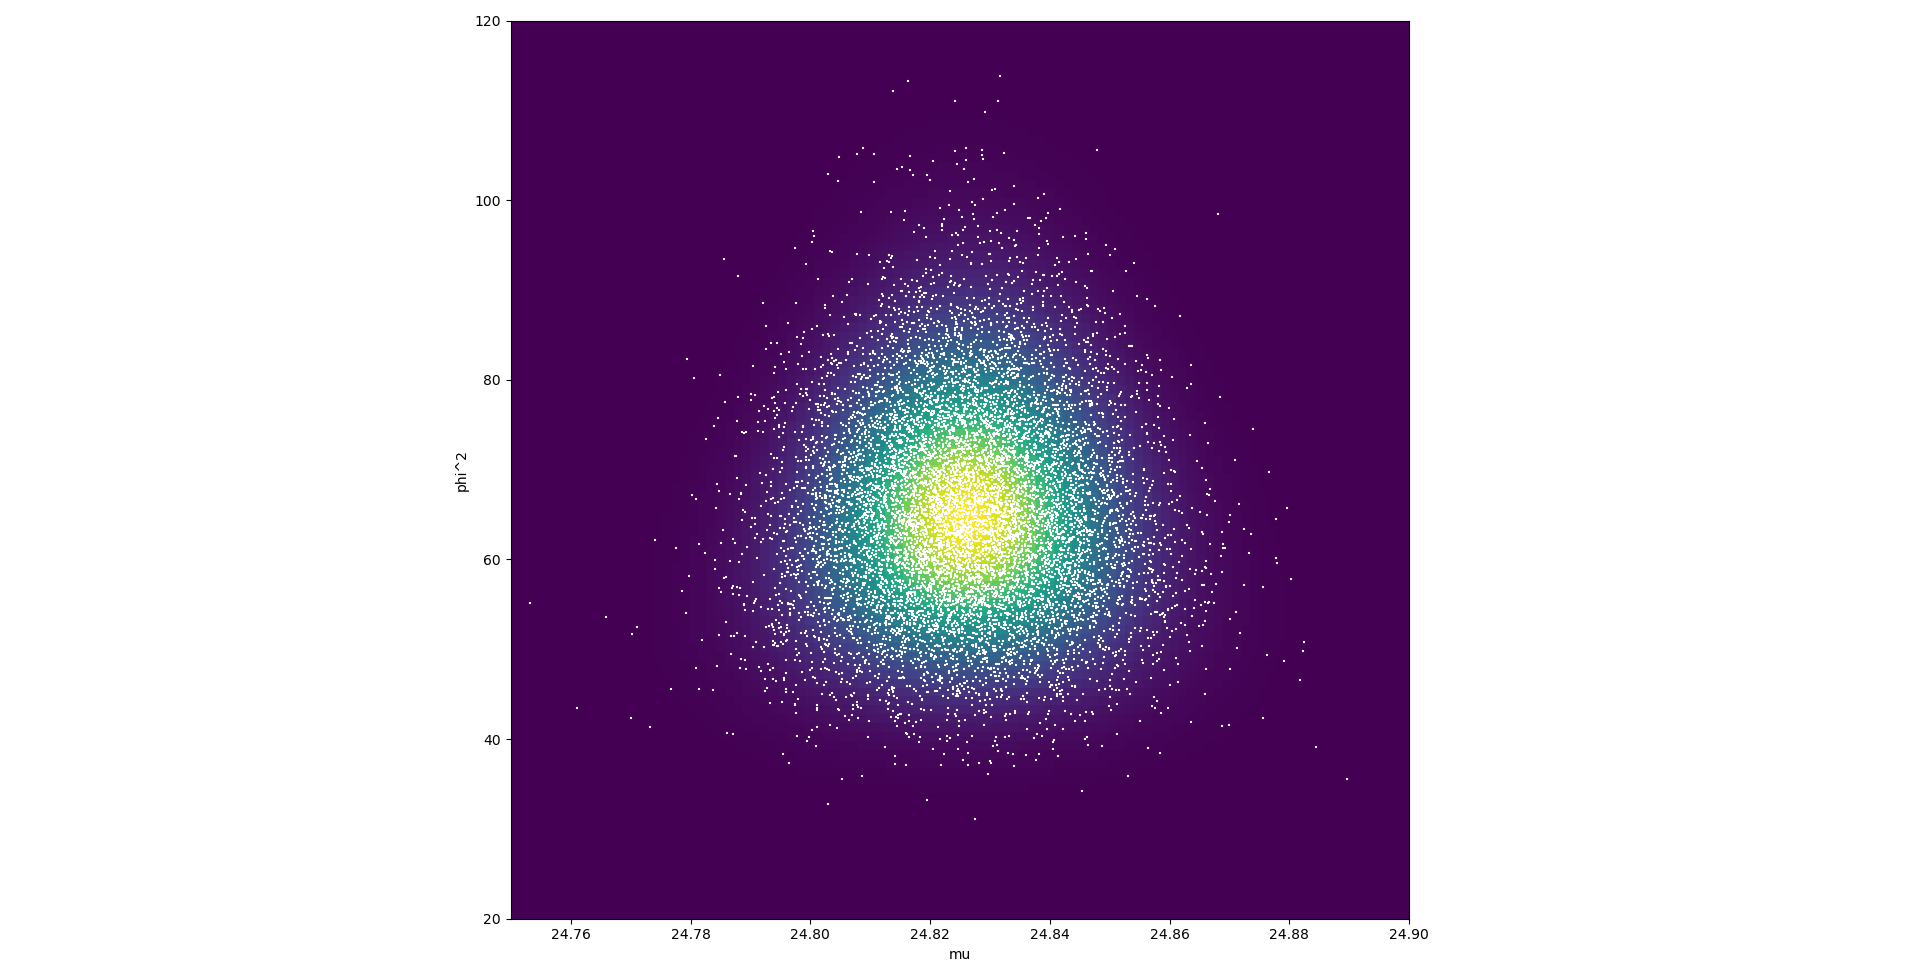
\includegraphics[width=0.5\textwidth]{STATS509/HW6/HW6Figures/problem5bi.png}
        \end{center}
    
        \item[(ii)] Find the $2.5\%$, $50\%$ and $97.5\%$ quantiles of the marginal posterior $p(\mu \mid y_1,\ldots ,y_n)$ (by finding these quantiles in your sample of $10,000$ draws).
        
        \lstinline[language=Python]{mu 25th 50th and 97.5th qunatiles: [24.79595245 24.8261025  24.85651072]}

        \item[(iii)] Find the $2.5\%$, $50\%$ and $97.5\%$ quantiles of the marginal posterior $p(\phi^2 \mid y_1,\ldots ,y_n)$ (again by using your $10,000$ draws).
        
        \lstinline[language=Python]{phi^2 25th 50th and 97.5th qunatiles: [45.1711972  64.86764863 89.2792161 ]}
    
        \item[(iv)] Find the $2.5\%$, $50\%$ and $97.5\%$ quantiles of the marginal posterior $p(\sigma \mid y_1,\ldots ,y_n)$ for the population s.d. 
        
        \lstinline[language=Python]{sigma_phi^2 25th 50th and 97.5th qunatiles: [0.1058339  0.12416121 0.14878844]}
    
        \item[(v)] As noted, the distance between Newcomb's lab and the mirror on the Washington Monument was $7.44373\; km$. Express the speed of light ($c$ in $km/s$) as a simple function of $\mu$. Use this information to find the $2.5\%$, $50\%$ and $97.5\%$ quantiles of the posterior $p(c \mid y_1,\ldots ,y_n)$ {\it Hint: this requires one line of R code using the vector of samples for $\mu$, which is stored in {\tt samples[,1]}.}
        
         \lstinline[language=Python]{c (km/s) quantiles: 2.994680e+05, 2.998348e+05, 3.001994e+05} \newline
         \lstinline[language=Python]{From sample mean c(km/s): 2.998334970980085e-07} \newline
        \lstinline[language=Python]{With sample std c(km/s): 0.0006980497158762172} 
    
        \item[(vi)] Compare your answer in (v) to the best current measurements of the speed of light. 
        
        Pretty close to current textbook values of 2.99792458e5 km/s.
    
        \item[(vii)] Look at a simple histogram of the observed data; compute the sample mean and sample standard deviation. Do you see anything that might make you question the assumption that the observations follow a normal distribution?
    
         \lstinline[language=Python]{Measured mean time: 24.826212121212123}\newline
         \lstinline[language=Python]{Measured mean std: 0.010663610099255412}
    
        \begin{center} 
            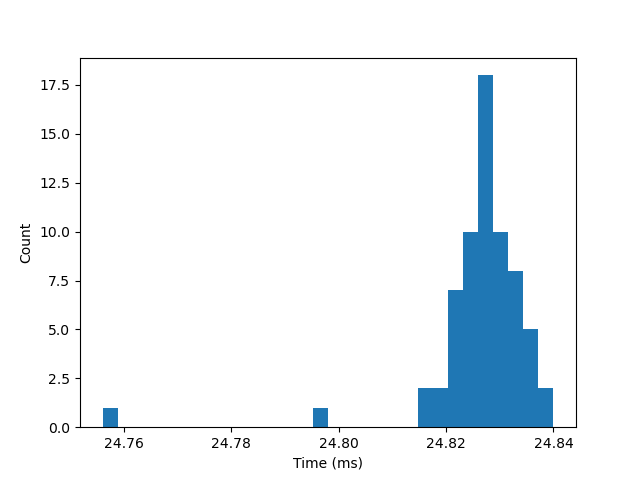
\includegraphics[width=0.5\textwidth]{STATS509/HW6/HW6Figures/problem5bvii.png}
        \end{center}
        
        The two largest outliers are significantly smaller than the measured mean making the sample distribution suspicious, but given that even in these outliers are in absolute terms very close to the mean I don't think it's a problem.
\end{enumerate}

{\it\scriptsize Note: the script contains various techniques for checking convergence of the Gibbs sampler, e.g. computing the auto-correlation and examining parallel boxplots. These can safely be ignored in this example!}
\end{enumerate}
{\small If you are interested, historical information on the Newcomb experiment is given here:
\hspace{-1cm}{\scriptsize \url{https://www.stat.washington.edu/tsr/s509/examples/newcomb/background-on-newcomb-experiment.pdf}}\par
}
\eject

\subsection*{Gibbs sampling}

This question provides intuition as to why Gibbs sampling works. The idea is that the `target distribution' that we wish to draw samples from (in Bayesian analyses this is the posterior distribution) is preserved by the steps in the procedure. (In more technical language, the procedure creates a Markov chain with a stationary distribution that is the target distribution.)

\subsection*{Problem 6.}
Consider the following joint density: Let  $X,Y$ be random variables with the following joint pdf:
\begin{equation}\label{eq:one}
    f_{XY}(x,y) = \left\{  \begin{array}{cl}
        2 &   0< x <1,\hbox{ and } 0 < y < x < 1 \\[5pt]
        0   & \hbox{otherwise,}
        \end{array}
    \right.
\end{equation}

\begin{enumerate}
    \item[(a)] Find the conditional densities $f(x\mid y)$ and $f(y \mid x)$.
    
    \begin{align*}
        f(x|y) = \frac{f(x,y)}{f(y)}& \\
        \\
        &f(y) = \int_y^1 f(x,y) dx \\
        &= \int_y^1 2dx \\
        &= 2(1-y) \\
        \\
        f(x|y) = \frac{2}{2(1-y)}&
    \end{align*}
    And the other way around:
    \begin{align*}
        &f(x) = \int_0^x f(x,y) dx = 2x \\
        \\
        f(x|y) = \frac{1}{x}&
    \end{align*}
    
    \newpage
    \item [(b)] Consider the following two step Gibbs simulation scheme for finding a new point $(X_{new}, Y_{new})$ given an existing point $(X_{old}, Y_{old})$:
    \begin{align*}
        X_{new} \sim&\quad X \mid Y_{old}\\
        Y_{new} \sim&\quad Y \mid X_{new}
    \end{align*}
    where these are the conditional distributions computed in (a).
    \begin{enumerate}
        \item[(i)] Show that if $(X_{old},Y_{old})$ has the joint density given by (\ref{eq:one}) then $(X_{new},Y_{old})$ also has the joint density  (\ref{eq:one}).\par
        {\it Hint: note that 
        $$f(x_{new},x_{old},y_{old}) = f(x_{new}\mid y_{old})f(x_{old},y_{old}),$$
        then integrate out $x_{old}$.}
        
        \begin{align*}
            f(x_n, y_o) &= \int_{y_o}^1 f(x_n|y_o)f(x_o,y_o)dx_o \\
            &= \frac{1}{1-y_o} \int_{y_o}^1 2 dx_o \\
            &= \frac{2}{1-y_o}(1-y_o) \\
            &=2
        \end{align*}

        \item[(ii)] Similarly show that if $(X_{old},Y_{old})$ has the joint density given by (\ref{eq:one}) then  $(X_{new},Y_{new})$ also has the joint density  (\ref{eq:one}).
        
        \begin{align*}
            f(x_n, y_n) &= \int_0^{x_n} f(y_n|x_n)f(x_n,y_o)dy_o \\
            &= \int_0^{x_n} \frac{1}{x_n} 2dy_o \\
            &= \frac{2}{x_n}\int_0^{x_n}dy_o \\
            &=2
        \end{align*}
    \end{enumerate}

    \newpage
    \item[(c)] A friend  suggests using the following sampling scheme instead:
    \begin{align*}
        X^*_{new} \sim &\quad  X \mid Y_{old}\\
        Y^*_{new} \sim &\quad Y \mid X_{old}
    \end{align*}
    Show that even  if $(X_{old},Y_{old})$ has the joint density given by (\ref{eq:one}), $(X^*_{new},Y^*_{new})$ does {\bf not} have the density (\ref{eq:one}). {\it Hint: consider the support of $(X^*_{new},Y^*_{new})$. It may also help to draw a picture.}
    
    \begin{align*}
        f(x^*_n, y^*_n) &= \int_{y^*_n}^1 \int_0^{x^*_n} f(y^*_n, x_o, y_o) dy_o dx_o \\
        &= \int_{y^*_n}^1 \int_0^{x^*_n} f(y^*_n|x_o, x^*_n, y_o) f(x_o, x^*_n, y_o) dy_o, dx_o \\
        &= \int_{y^*_n}^1 \int_0^{x^*_n} f(y^*_n|x_o) f(x_o, x^*_n, y_o) dy_o dx_o\\
        &= \int_{y^*_n}^1 \int_0^{x^*_n} f(y^*_n|x_o) f(x^*_n|y_o) f(x_o, y_o) dy_o, dx_o\\
        &= \int_{y^*_n}^1 f(y^*_n|x_o) \int_0^{x^*_n} f(x^*_n|y_o) f(x_o, y_o) dy_o, dx_o \\
        &=  \int_{y^*_n}^1 f(y^*_n|x_o) dx_o \frac{2}{x^*_n} x^*_n\\
        &= 2 \int_{y^*_n}^1 \frac{1}{x_o} dx_o \\
        &= -2 \ln{y^*_n}
    \end{align*}
\end{enumerate}



\newpage
\subsection*{Sampling Distributions}
Questions from Goldberger:

\subsection*{Problem 7}
Qu.~8.3 (This is review of material from Chapters 2 and 3.)

\begin{enumerate}
    \item Bernouli with $p=0.5$
    
    \begin{align*}
        E[X] &= 0.5 \\
        V[X] &= 0.5(1-0.5) = 0.25 \\
        P(A) &= P(0.4\leq X \leq 0.6) = 
    \end{align*}
    
    \item Normal with parameters $\mu=0.5$ and $\sigma^2=0.25$
    
    \begin{align*}
        E[X] &= 0.5 \\
        V[X] &= 0.25 \\
        P(A) &= P(0.4\leq X \leq 0.6) = 0.159
    \end{align*}
    
    \item Exponential with $\lambda=2$
    
    \begin{align*}
        E[X] &= 0.5 \\
        V[X] &= 0.25 \\
        P(A) &= P(0.4\leq X \leq 0.6) = 0.148
    \end{align*}
\end{enumerate}


\newpage
\subsection*{Problem 8}
Qu.~8.4  (See section 8.3 on p.85.)

From section 8.3 we have that:
\begin{enumerate}
    \item if $X\approx$Bernoulli, then $n\bar X\approx$Binomial(n,p)
    \item if $X\approx$Normal, then $\bar X\approx$Normal($\mu, \sigma^2/n$)
    \item if $X\approx$Exponential, then $2n\lambda \bar X\approx$Chi-square(k)
\end{enumerate}
 n=10
 
\begin{enumerate}
    \item Bernoulli with $p=0.5$
    
    \begin{align*}
        E[\bar X] &= 0.5 \\
        V[\bar X] &= 0.5(1-0.5) = 0.025 \\
        P(A) &= P(0.4\leq X \leq 0.6) = 0.451
    \end{align*}
    
    \item Normal with parameters $\mu=0.5$ and $\sigma^2=0.25$
    
    \begin{align*}
        E[\bar X] &= 0.5 \\
        V[\bar X] &= 0.025 \\
        P(A) &= P(0.4\leq X \leq 0.6) = 0.451
    \end{align*}
    
    \item Exponential with $\lambda=2$
    
    \begin{align*}
        E[\bar X] &= 0.5 \\
        V[\bar X] &= 0.25 \\
        P(A) &= P(0.4\leq X \leq 0.6) = 0.451
    \end{align*}
\end{enumerate}

\newpage
\subsection*{Problem 9}
Goldberger Qu. 8.7\par
{\it Hint: For part (b) read pages 87-88, Section 8.5.}

\begin{enumerate}
    \item The function $Y$ is concave. So by Jensen's inequality we have
    
    $$E[g(X)] \leq g\left( E[X] \right)$$
    Given is that $E[\bar X] = 1/\lambda$ so $1/E[\bar X] = \lambda$. Applying Jensen's inequality to the problem then yields:
    
    $$\lambda = \frac{1}{E[\bar X]} \leq E\left[\frac{1}{\bar X}\right] = E[T]$$
    
    \item If $\lambda =2$ and $n=10$ find E(T) and V(T):
    From problem 8 we know that if X~Exponential then $2n\lambda\bar X \approx$ Chi-Square(2n) so we define $W=2n\lambda\bar X \approx \chi^2(2n)$ and look for:
    \begin{align*}
        E[1/W] &= E\left[ \frac{1}{2n\lambda\bar X} \right] \\
        &= \frac{1}{2n\lambda} E\left[ \frac{1}{\bar X} \right] \\
        &= \frac{1}{2n\lambda} E[T] \\
        E[T] &= 2n\lambda E[1/W] \\
        &= \frac{2n\lambda}{2n -2} \\
        &= \frac{40}{18} \approx 2.222\hdots
    \end{align*}
    
    and the variance:
    \begin{align*}
        E[1/W^2] &= E\left[ \frac{1}{4n^2\lambda^2\bar X^2} \right] \\
        &= \frac{1}{4n^2\lambda^2} E\left[ \frac{1}{\bar X^2} \right] \\
        &= \frac{1}{4n^2\lambda^2} E[T^2] \\
        E[T^2] &= 4n^2\lambda^2 E[1/W^2] \\
        &= \frac{4n^2\lambda^2}{(2n -2)(2n-4)} \\
        &= \frac{1600}{288} \approx 5.5555\hdots
    \end{align*}
    $$\rightarrow V[T] = E[T^2] - E[T]^2 \approx 3.3333\hdots$$
    Where we used the expectation values of inverse Chi-square RV found in the book chapter 8.5 (page 88). 
\end{enumerate}


\end{document}
